\chapter{Preparation}\label{ch:preparation}
Before powering the \gls{tlu} it is necessary to follow a few steps to ensure the board and the \gls{fpga} work correctly.\\
The \brd is designed to plug onto a carrier \gls{fpga} board like any other \gls{fmc} mezzanine board, although its form factor does not comply with the ANSI-VITA-57-1 standard.\\
The firmware developed at University of Bristol is targeted to work with the Enclustra  AX3 board, which must be plugged onto a PM3 base, also produced by \href{http://www.enclustra.com/en/home/}{Enclustra}. The firmware is written on the \gls{fpga} using a \gls{jtag} interface. Typically a breakout board will be required to connect the Xilinx programming cable to the Enclustra PM3.\\
Currently, it is recommended to use the following:
\begin{itemize}
 \item MA-PM3-W-R5: Mars PM3 base board
 \item MA-AX3-35-1I-D8-R3: Marx AX3 module (hosts a Xilinx XC7A35T-1CSG324I )
 \item MA-PM3-ACC-BASE: Accessory kit, including a \gls{jtag} breakout board to connect Xilinx programming cables. Also includes a 12~V power supply to power the PM3.
\end{itemize}

\section{I/O voltage setting}
The I/O pins of the PM3 can be configured to operate at 2.5~V or 3.3~V; the factory default is 2.5~V but the \brd requires 3.3~V logic. The user should make sure to select the appropriate voltage by operating on DIP-switch CFG-A/S1200 (pin 1 set to ON).\\For reference, a top view of the board is provided in the appendix at page~\pageref{ch:appendix}.\\
\begin{alertinfo}{Warning}
    Please double check the PM3 board manual for the correct way to change the I/O voltage setting. Enclustra has been changing their hardware recently.
\end{alertinfo}

\section{Xilinx programming cable}
The \gls{jtag} pins on the PM3 are located on the header J800 (20-way, 2.54~mm pitch). The breakout board provided by Enclustra sits on top of the header and connects the pins to a 14-way Molex milli-grid header so that it is possible to plug the Xiling programming cable directly onto it. However, when the \brd is mounted on a base plate as shown in figure~\ref{fig:TLUplate}, the breakout board has to be detached from the PM3 because it interferes with the mounting screws.\\
The connection between J800 and the breakout can be achieved by using two standard 20-way \gls{idc} cables as shown in figure~\ref{fig:XilinxCable}.
\begin{figure}[h]
  \centering
  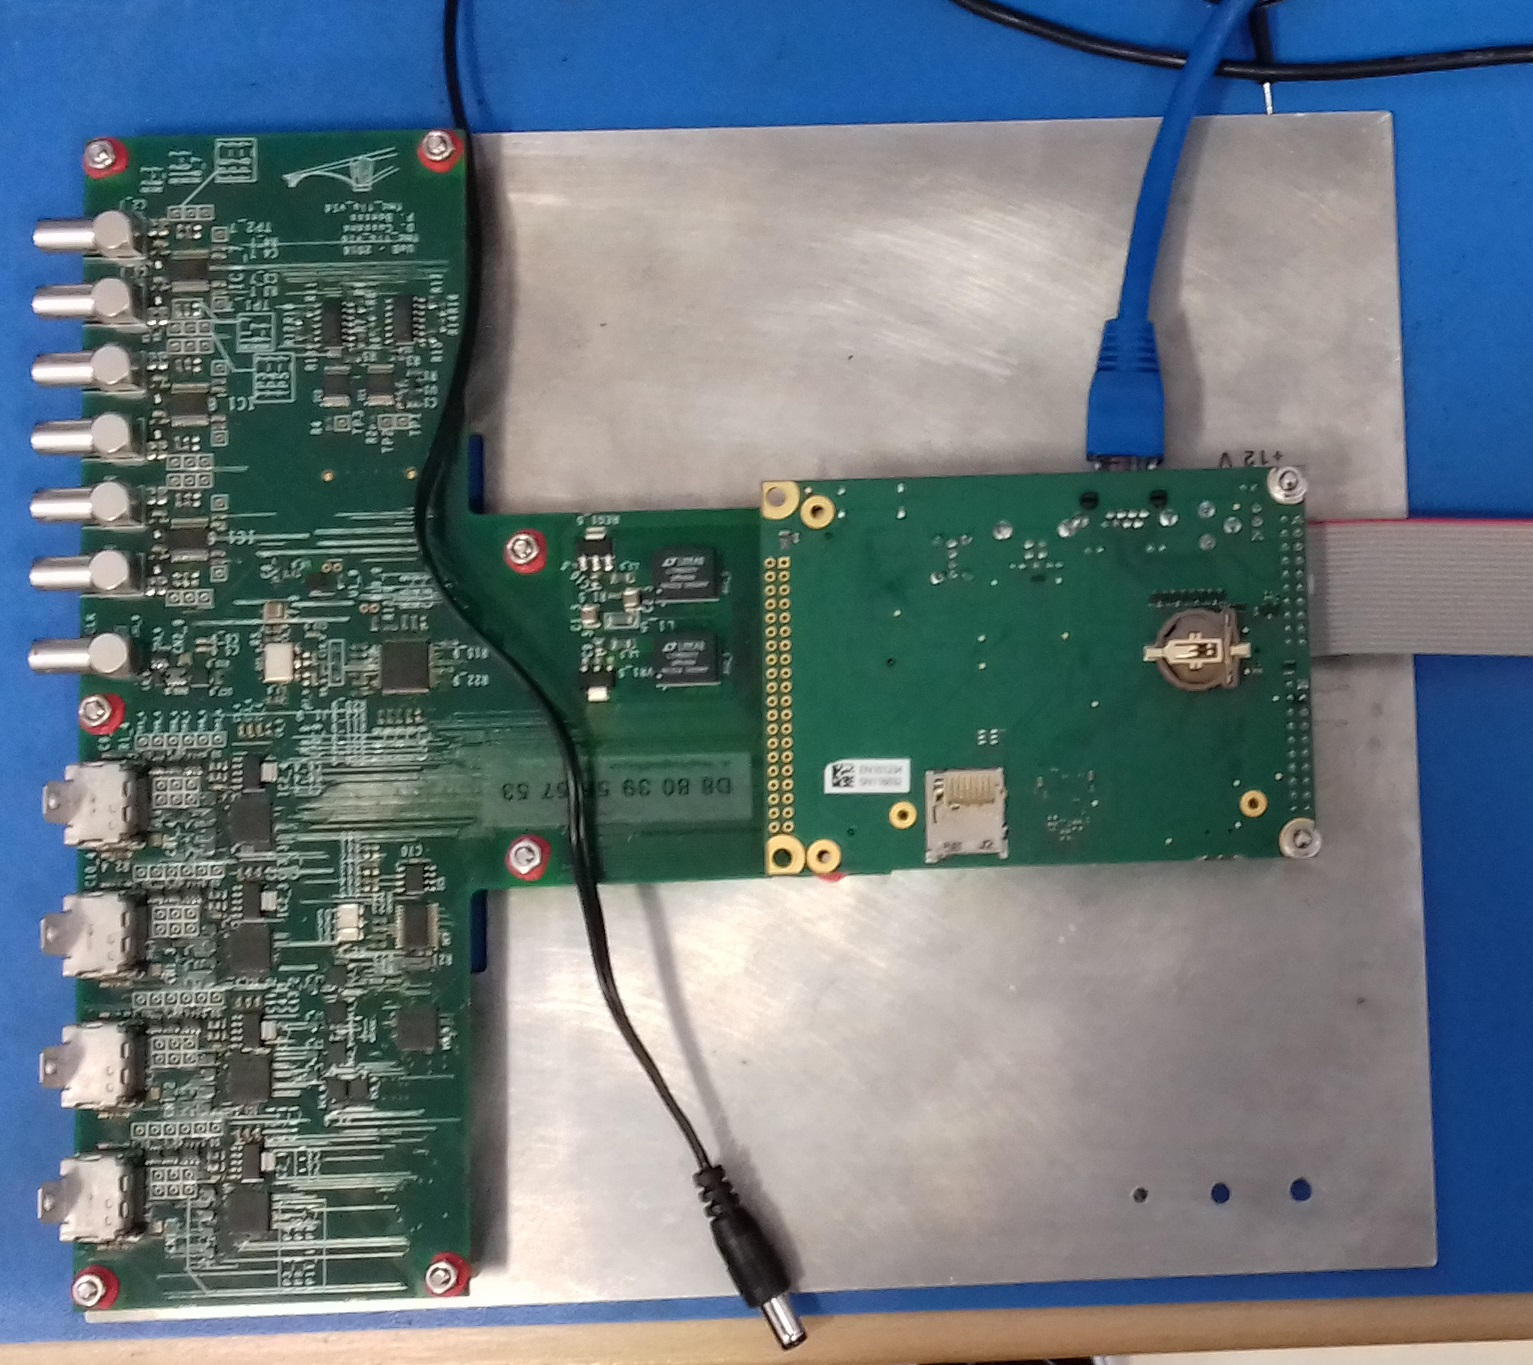
\includegraphics[width=.50\textwidth]{./Images/TLU_plate.jpg}
  \caption{\brd and PM3 mounted on a base plate: in this configuration it is not possible to install the breakout board on the PM3 because the mountings screws are in the way.}\label{fig:TLUplate}
\end{figure}
\begin{figure}
  \centering
  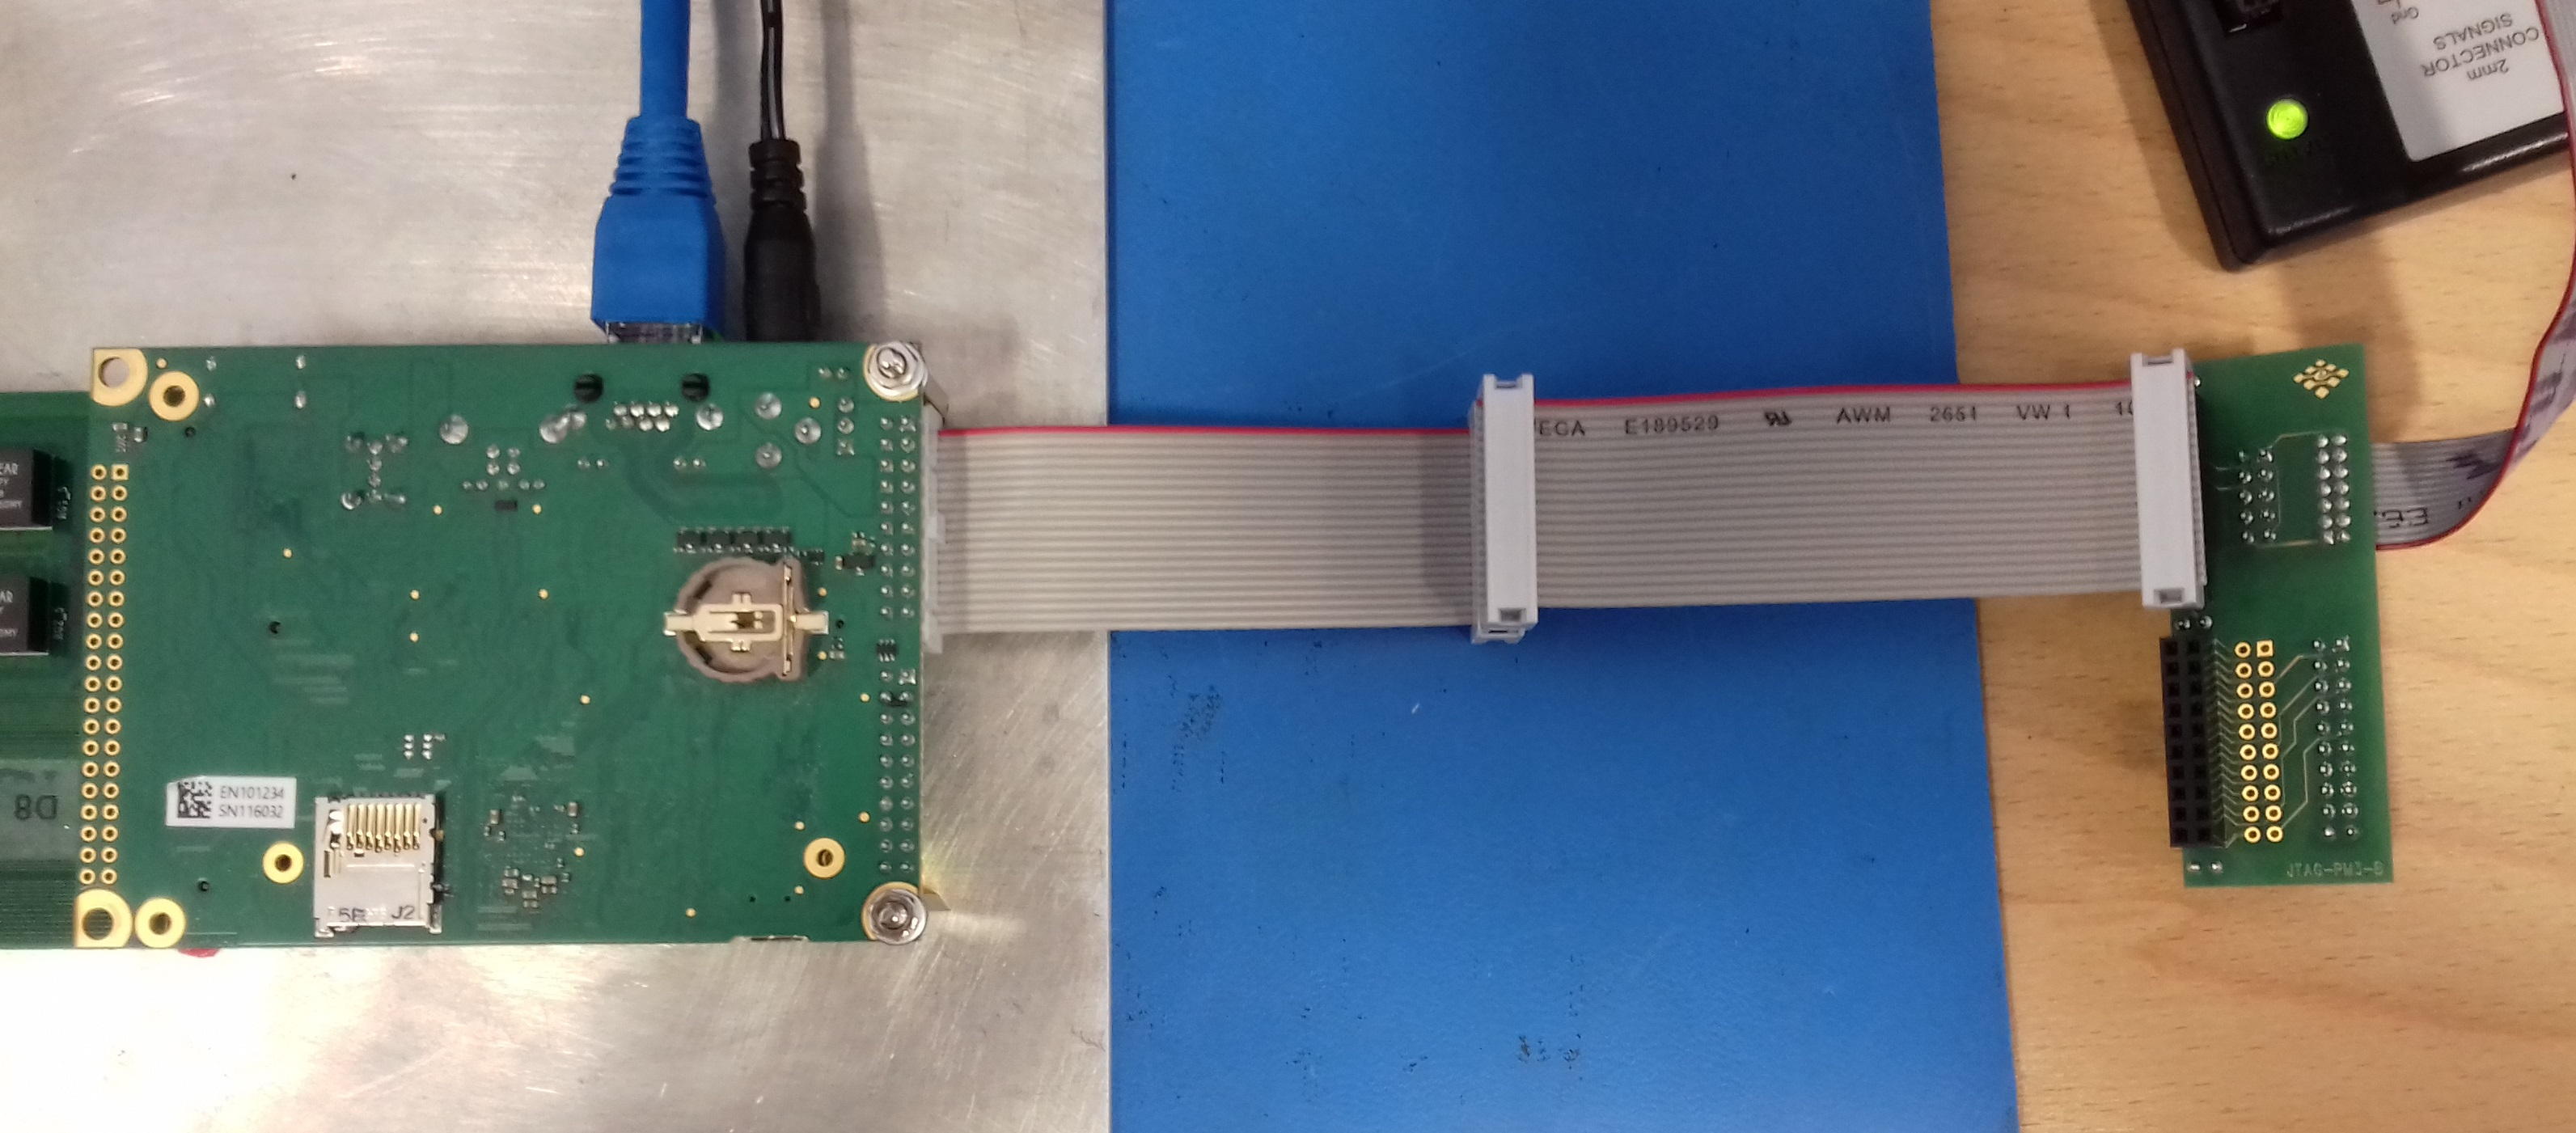
\includegraphics[width=.80\textwidth]{./Images/XilinxCable.jpg}
  \caption{Connecting the Xilinx programming cable to the PM3 in an ugly (but effective) way.}\label{fig:XilinxCable}
\end{figure}
